\subsection{Essentials of probability theory and graph theory}
% 1.5 pages

\subsubsection{Probability theory}

The domain on probabilistic models is the probability theory. Probability describes how likely one beliefs that an event of uncertain nature occurs. By conducting multiple experiments or observing the behavior of a system, such probabilities can be estimated.

Because of the limited view onto a natural system, that humans or computers can have, probabilistic models are used to represent the main aspects of such system with uncertain events. Therefore a event space $\Omega$ is defined. $\Omega$ is a set of all possible outcomes of an event like rolling a die, $\Omega=\{1,2,3,4,5,6\}$.

In order to quantify the belief in how likely an outcomes emerges, a real number between zero and one, called probability, is assigned to each outcome, such that the sum of the probabilities of all outcomes is equal to one. This assignment is called probability distribution.

Upon random experiments random variables are defined, which might represent single possible outcomes of the event space or a more complex combination. They are used in order to formulate questions of inference. For example, how likely is it, that the sum of three dies is equal to four. The random variable $X$ hereby would be the sum of numbers on three dies after rolling them. The probability would be written as $P(X=4)$. Hereby $4$ is one value of $X$. The values of a random variable $X$ is often denoted as $x_1, x_2,  ..., x_n$, if there are n possible values.

Furthermore dependences or independences among random variables are important for inference. If it is known that one variable $A$ is independent from another variable $B$, it is not necessary to care about the $B$ when inferring about the probabilities of the values of $A$. $A$ is independent of $B$ if the probability distribution of $A$ does not change, whatever value $B$ attains.

In order to simplify probabilistic inference on large models, where we have a lot of random variables and dependencies, graphical models are used, as being discussed in sections \ref{sec:introugm} and the following.

\subsubsection{Graph theory} \label{sec:graph}

The second theoretical foundation of probabilistic graphical models is the graph theory. Graphs are used to represent and also illustrate a large variety of models, like also probabilistic models.

The basic components of a graph are a set of nodes and a set of edges, which represent relation between the nodes. In case of probabilistic models nodes represent random variables and edges represent the dependency between two random variables. An edge is a pair of nodes, which in the case of an directed edge needs to be ordered. If the graph is undirected the pairs of nodes have not necessarily to be ordered. This project paper mainly refers to undirected graphs.

Depending on the model graphs can be large and often only a restricted scope is needed to answer a certain question of interest. Therefore subgraphs are defined, such that the nodes of a subgraph is a subset of nodes of the original graph and the set of edges are all edges of the original graphs, whose nodes are also included in the subset of nodes. For example if their is a graph of relationships among students of an university and the question is how many relationships exists in a certain course, only the subgraph of the course is needed to answer the question. This might save computation time and space.

Furthermore a path from node $A$ to node $Z$ is a set of edges, such which connects those nodes $\{(A,B),(B,C),...,(Y,Z)\}$. If there is a path from one node to another in an undirected graphical model, those variables are at least indirectly dependent on each other.
% TODO: is that true???

If there is a path, where the starting point is the same as the end point without using an edge multiple times, this path is considered to by a cycle. As is described in section \ref{sec:bayes} Bayesian networks are not allowed to have cycles, whereas cycles can be represented in undirected graphical models.

\subsection{Introduction to undirected graphical model} \label{sec:introugm}
% 0.5 pages

\cite{hammersley1971markov}
\cite{pearl2014probabilistic}

As already described in section \ref{sec:graph}, in undirected graphical models nodes represent random variables and edges represent the dependences among those variables. Since the purpose of an undirected graphical model is to represent undirected mutual dependences between two variables at a time, the edges of the graph are also undirected. Probabilistic undirected graphical models are also called Markov networks or in some areas of application Markov random field, as is described in section \ref{sec:application}.

The following example should illustrate a simple probabilistic model which is represented in a Markov network: Let there be four people $A$, $B$, $C$ and $D$, whereby it is unknown if their are vegetarian or not. Thus, their are four binary random variables. Furthermore it is known, that it is more likely that people that know each other are more likely to have the same eating habits than different ones. It is assumed that knowing people is mutual and not directed. As shown in \ref{fig:basic} $C$ knows all, $D$ only knows $C$, $A$ knows $B$ and $C$ and $B$ knows $A$ and $C$. In order to infer new knowledge on this Markov network and actually calculate probabilities, the Markov network requires a quantification of affinities among the nodes, which will be discussed in the next section (\ref{sec:param}). In other words, how likely is it, that for example $A$ and $B$ both are vegetarian or that $A$ is vegetarian and $B$ is not.

\begin{figure}[htpb]
  \centering
  	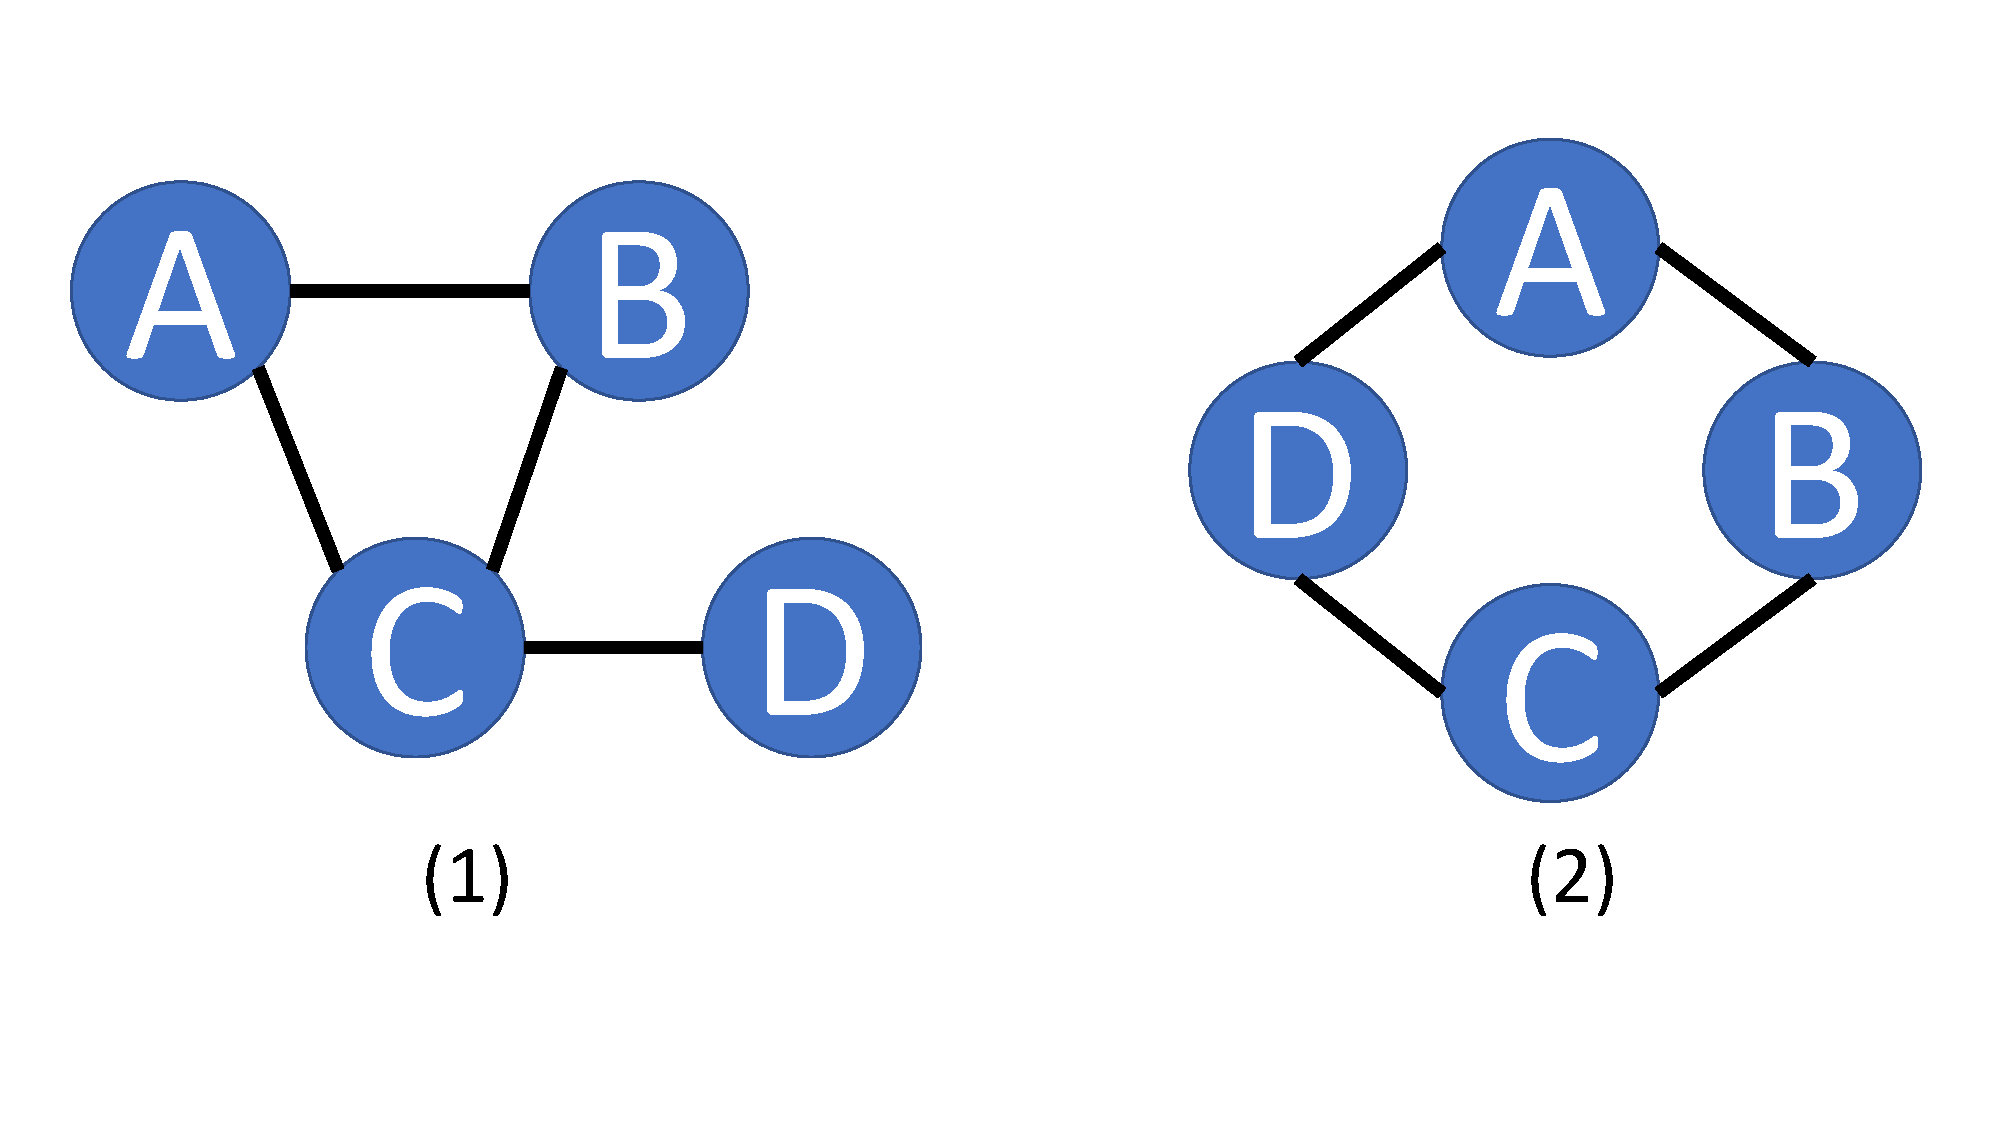
\includegraphics[scale=0.3]{img/basic.pdf} 
  \caption{Simple Undirected Graphical Model}
  \label{fig:basic}
\end{figure}

\subsection{Parameterization} \label{sec:param}
% 2 pages

% TODO: short outlook into overparameterization

In order to conduct inference and learning on an Markov network, the model needs to be parameterized in the first place. Hereby the goal is to quantify the affinity, how likely the assignments of dependent variables are. The parameterization is achieved by assigning factors to subsets of random variables of the graph. The subsets needs to be cliques, which mean that each node in the clique depends on every other node in the clique. Each factor includes multiple parameters, which assign a real number to a certain combination of values of the random variable of the factors scope. For example, let $A$ and $B$ are binary random variables, which mutually depend on each other, their is a factor $\phi(A,B)$, which includes one parameter per assignment $\{(a_0,b_0),(a_0,b_1),(a_1,b_0),(a_1,b_1)\}$ . In contrary to the conditional probability distribution, which is used with Bayesian networks, as described in section \ref{sec:bayes}, the sum of assigned real numbers of a parameter do not necessarily need to sum up to one, because they do not directly represent probabilities but compatibilities amongst the nodes of the factor.

Figure \ref{fig:param} shows a factor of two dependent binary random variables and demonstrate the assignment of compatibility to each parameter.

\begin{figure}[htpb]
  \centering
  	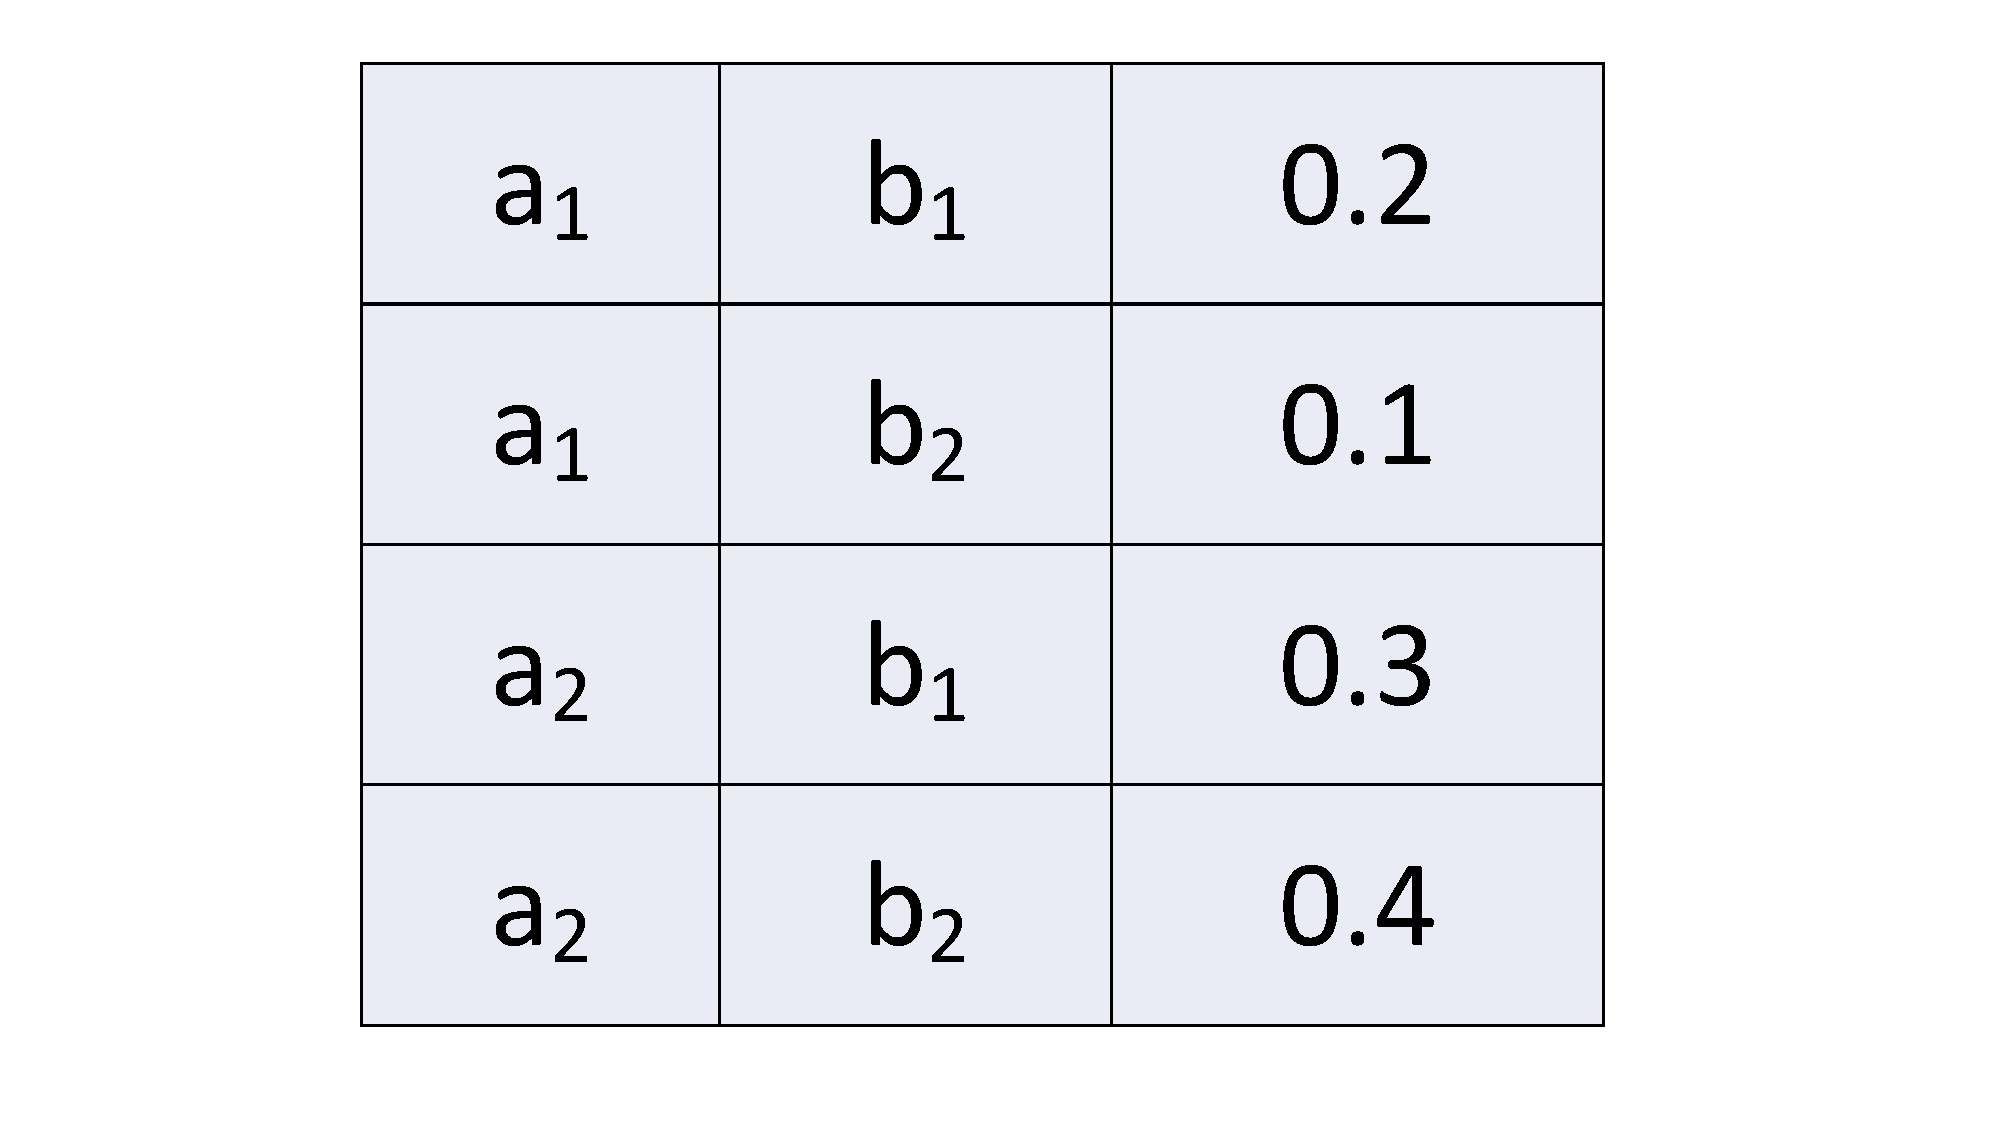
\includegraphics[scale=0.3]{img/param.pdf} 
  \caption{Factor of two binary linked random variables}
  \label{fig:param}
\end{figure}

In order to obtain the compatibility scores of assignments of all nodes, all factors are combined with a factor multiplication. Hereby the values of the parameters across the factors are multiplied in a way, that the assignments of the random variables match up. Thus, if $A$ and $B$ is one clique with $\Phi(A,B)$ and $B$ and $C$ is another clique with $\Phi(B,C)$, then $\Phi(A,B,C)=\Phi(A,B)\times\Phi(B,C)$. Figure \ref{fig:parammult} shows an example of a factor multiplication of factors with random variables. If all parameters are strictly positive than this distribution is also considered a Gibbs distribution, as described in \cite{kindermann1980markov}.

An important aspect of the resulting factor is that the number of parameters increased. While the two original factors $\Phi(A,B)$ and $\Phi(B,C)$ had in total ten parameters, the new factor $\Phi(A,B,C)$ contains twelve parameters. So if there are $n$ binary variables and each factor is defined on two variables, the number of parameters of the single factors would be $4\times n$ but the number of parameters of the factor product of all factors would be $2^n$, which leads to more computational space and time while processing a large model with many random variables. Section \ref{sec:indep} describes how independences and given values of random variables, help to reduce the scope of factor multiplications.

Besides the number of parameters the factor multiplication delivers also unnormalized compatibility scores and not probabilities. To achieve a probability distribution the scores needs to be normalized by the sum of all scores. How inference is possible with this probability distribution is discussed in section \ref{sec:infer}.

% TODO: image: use a,b,c like in the book and do unnormalized and normalized, like in the book

\begin{figure}[htpb]
  \centering
  	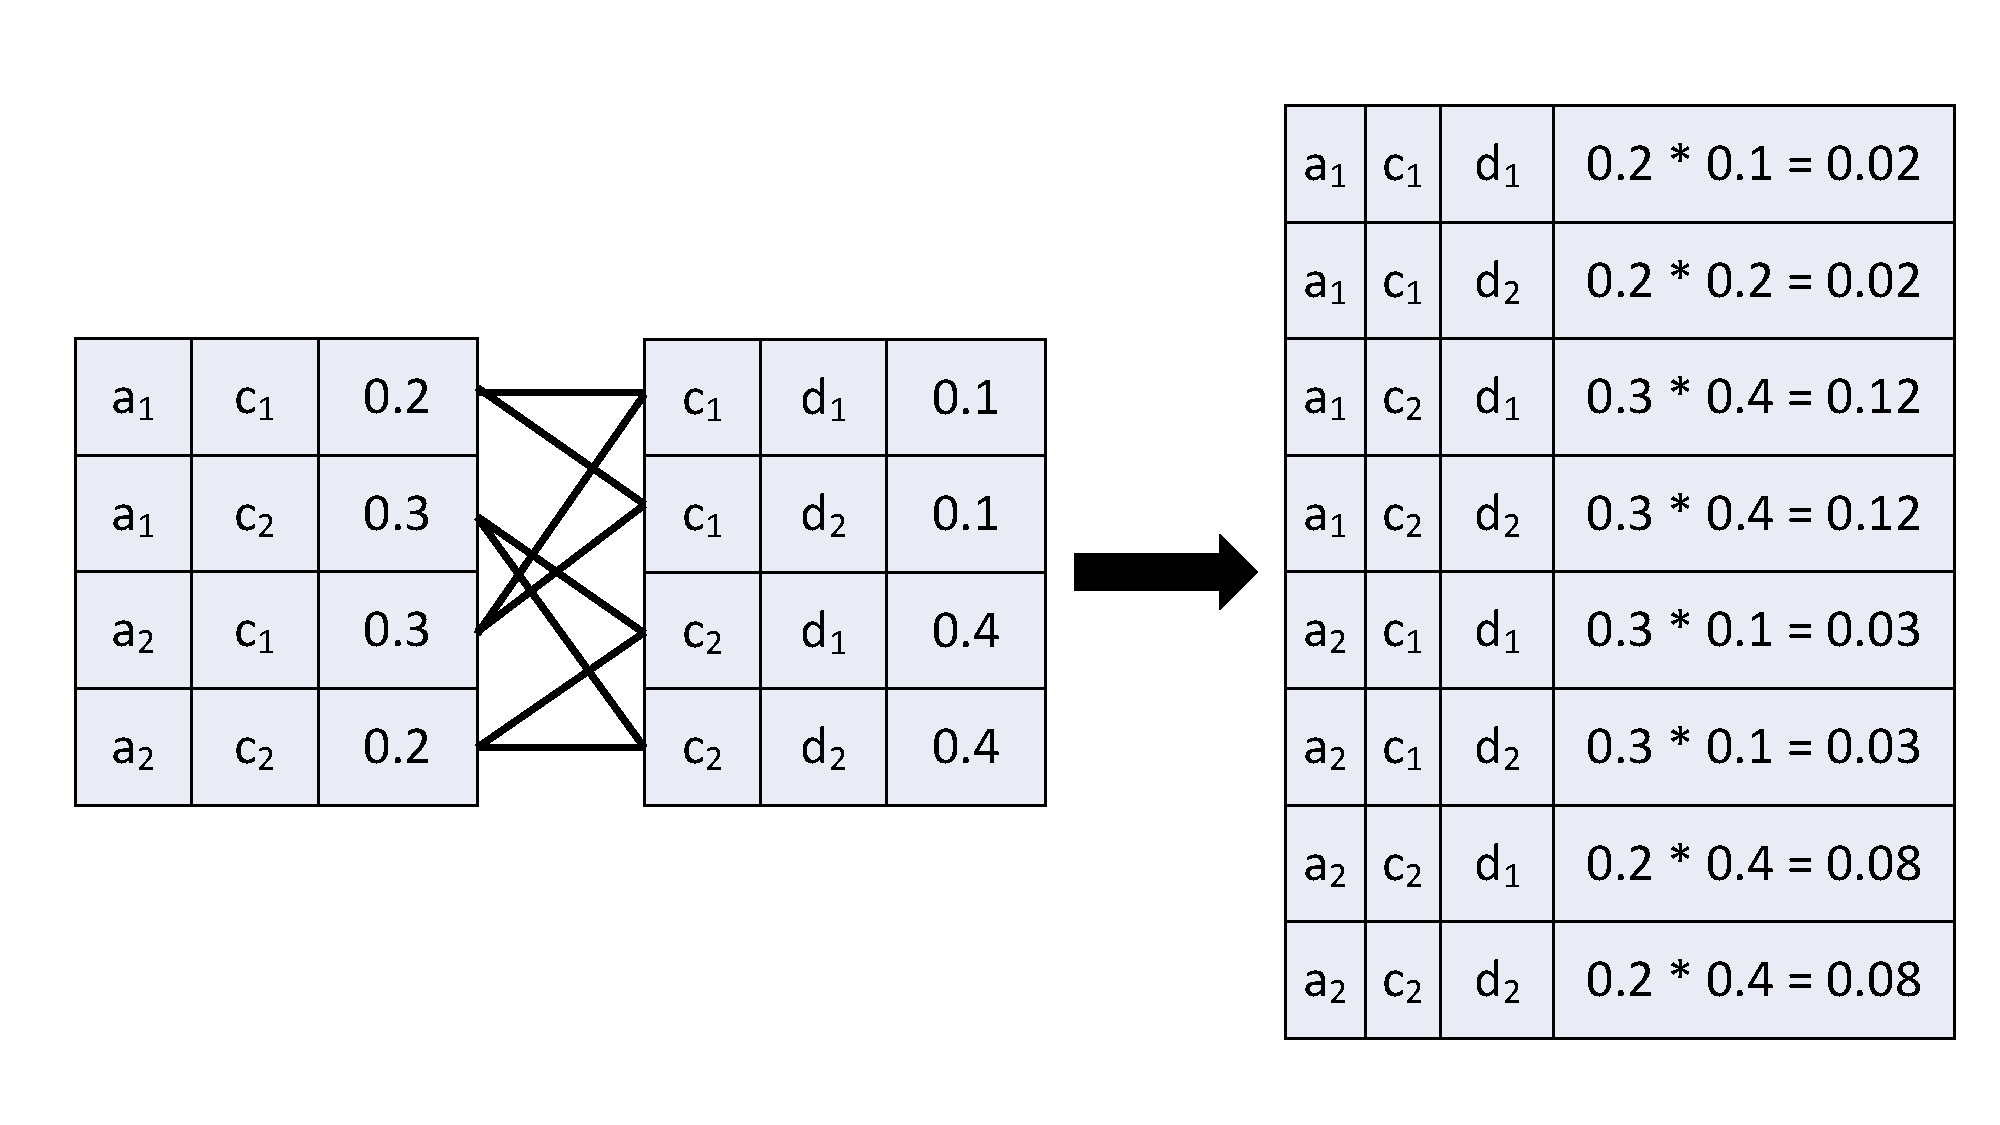
\includegraphics[scale=0.4]{img/parammult.pdf} 
  \caption{Factor multiplication of three binary random variables}
  \label{fig:parammult}
\end{figure}

% TODO Parameterization revisited: log-linear models

- clique potentials are often replaced by an exponentiated sum of features times their weights in log linear models
- this features are used in Markov logic networks, as discussed in section \ref{sec:mln}

\subsection{Independences in Markov networks} \label{sec:indep}
% 0.5 page

As described in section \ref{sec:introugm} the Markov network is supposed to represent the dependencies of a model. Since the dependencies are mutual, they flow along every direction through the graph, such that if there is a graph, in which there is a path from each node to every other node, all variables are indirectly dependent on each other, under the condition that their are no fixed assignments yet. In the contrary if there is a condition on a variables, the dependency "flow" stops right at this node.

From that the Markov properties are derived: the pairwise, local and global Markov property. The global Markov property states, that if there is a Markov network with a set of nodes $\mathbf{V}$ and two distinct subsets of nodes of $\mathbf{V}$ ($\mathbf{A}, \mathbf{B} \subset \mathbf{V} \wedge \mathbf{A} \cap \mathbf{B} = \emptyset$), and a third subset $\mathbf{C}$ that is also distinct from $\mathbf{A}$ and $\mathbf{B}$, the values of all its nodes are known and every path from a node of $\mathbf{A}$ to a node of $\mathbf{B}$ passes a node of $\mathbf{C}$, then all nodes of $\mathbf{A}$ are independent from all nodes of $\mathbf{B}$ and vise versa. This means, if there is a very large Markov network in practice and the need of inferring over a node, the computational effort in time and disc space can be dramatically reduced by finding such separating given subsets. This holds also for the local and the pairwise Markov property.

The local Markov property states, that if all adjacent nodes of a target node are given the target node is independent from all other nodes in the model. This set of adjacent nodes is also called Markov blanket and is also used in Bayesian networks, but with a different definition, as is described in section \ref{sec:bayes}. Finally the pairwise Markov property states, that two non-adjacent nodes are independent from each other, if all other nodes of the network are given. To be considered a Markov network the model needs to satisfy those three Markov properties, as described in \cite{markov1957theory}.


\subsection{Inference on undirected models} \label{sec:infer}
% 1 page

The goal of inference in probabilistic models is to gain knowledge like about unknown random variables. This section briefly discusses inferring knowledge about unknown variables, called query variables $Y$, given evidence $E=e$ in the form of known variables $P(Y|E=e)$ in Markov networks. Thus the result is a probability distribution over a set of query variables given a set of known variables. The set of query and the set of evidence variables are subsets of the set of all variables of the graph $Y,E \subset \mathcal{X}$.

Since the interrogation is a conditional probability, the definition can be applied:

\begin{equation}
P(\mathbf{Y}\ |\ E=e)=\frac{P(\mathbf{Y},e)}{P(e)}
\end{equation}

The probability $P(y,e)$ for a specific value $y \in Val(\mathbf{Y})$ can be computed by summing out all parameters of the full joint distribution where $y$ and $e$ matches the corresponding values in the distribution, as described in equation \ref{eq:sum}. Regarding Markov networks this would mean to sum out the normalized distribution.

\begin{equation}
P(y,e)=\sum_w{P(y,e,w)},\ with\ \mathbf{W} = \mathcal{X} - \mathbf{V} - \mathbf{E}
\label{eq:sum}
\end{equation}

Hereby the independences, described in section \ref{sec:indep}, are useful in order to reduce the amount of factors, which are needed to compute the sufficient joint distribution. Thus, computational costs can be dramatically reduced, if the evidence cuts of large parts of the graph.

In any case, this approach is not efficient in terms of complexity. As described in section \ref{sec:param} the number of parameters in the full joint distribution increases exponentially with increasing random variables. To solve this problem algorithm were found, which either enable exact or approximated inference on Markov networks.

An exact algorithm for inference on Markov networks is the variable elimination.

%- not efficient, NP-hard $\Rightarrow$ worst case exponential
%- variable elimination:
% - basic idea: eliminating a variable by summing out
% - given a set of variables and a subset X $\Rightarrow$ $\Phi(X,Y)$ %$\Rightarrow$ sum over values of Y $\Rightarrow$ generate factor of X without Y
% - ref to a table picture % like in p.297
% - how does this reduce complexity?
% - how to chose variable to eliminate?

% sources: https://en.wikipedia.org/wiki/Variable_elimination
% https://www.youtube.com/watch?v=jz02X3hByac

%- Clique trees % short description of the approach chapter 10

%- Approximate target distribution % short description of the approach chapter 11
% - energy functional % section 11.2
% - propagation-based algorithm % section 11.3

%- MAP and maximum-likelihood

\subsection{Learning undirected models}
% 1 page

\subsubsection{Motivation and Goals for learning probabilistic models}
% 0.5 pages
- [chapter 16]
- predictions, estimations

\subsubsection{Likelihood function for learning}
% 0.5 pages

- what is it
- what methods, how does this satisfy the goals
- specialty in comparison with Bayesian network
- outlook